% Options for packages loaded elsewhere
% Options for packages loaded elsewhere
\PassOptionsToPackage{unicode}{hyperref}
\PassOptionsToPackage{hyphens}{url}
\PassOptionsToPackage{dvipsnames,svgnames,x11names}{xcolor}
%
\documentclass[
  letterpaper,
  DIV=11,
  numbers=noendperiod]{scrartcl}
\usepackage{xcolor}
\usepackage{amsmath,amssymb}
\setcounter{secnumdepth}{-\maxdimen} % remove section numbering
\usepackage{iftex}
\ifPDFTeX
  \usepackage[T1]{fontenc}
  \usepackage[utf8]{inputenc}
  \usepackage{textcomp} % provide euro and other symbols
\else % if luatex or xetex
  \usepackage{unicode-math} % this also loads fontspec
  \defaultfontfeatures{Scale=MatchLowercase}
  \defaultfontfeatures[\rmfamily]{Ligatures=TeX,Scale=1}
\fi
\usepackage{lmodern}
\ifPDFTeX\else
  % xetex/luatex font selection
\fi
% Use upquote if available, for straight quotes in verbatim environments
\IfFileExists{upquote.sty}{\usepackage{upquote}}{}
\IfFileExists{microtype.sty}{% use microtype if available
  \usepackage[]{microtype}
  \UseMicrotypeSet[protrusion]{basicmath} % disable protrusion for tt fonts
}{}
\makeatletter
\@ifundefined{KOMAClassName}{% if non-KOMA class
  \IfFileExists{parskip.sty}{%
    \usepackage{parskip}
  }{% else
    \setlength{\parindent}{0pt}
    \setlength{\parskip}{6pt plus 2pt minus 1pt}}
}{% if KOMA class
  \KOMAoptions{parskip=half}}
\makeatother
% Make \paragraph and \subparagraph free-standing
\makeatletter
\ifx\paragraph\undefined\else
  \let\oldparagraph\paragraph
  \renewcommand{\paragraph}{
    \@ifstar
      \xxxParagraphStar
      \xxxParagraphNoStar
  }
  \newcommand{\xxxParagraphStar}[1]{\oldparagraph*{#1}\mbox{}}
  \newcommand{\xxxParagraphNoStar}[1]{\oldparagraph{#1}\mbox{}}
\fi
\ifx\subparagraph\undefined\else
  \let\oldsubparagraph\subparagraph
  \renewcommand{\subparagraph}{
    \@ifstar
      \xxxSubParagraphStar
      \xxxSubParagraphNoStar
  }
  \newcommand{\xxxSubParagraphStar}[1]{\oldsubparagraph*{#1}\mbox{}}
  \newcommand{\xxxSubParagraphNoStar}[1]{\oldsubparagraph{#1}\mbox{}}
\fi
\makeatother


\usepackage{longtable,booktabs,array}
\usepackage{calc} % for calculating minipage widths
% Correct order of tables after \paragraph or \subparagraph
\usepackage{etoolbox}
\makeatletter
\patchcmd\longtable{\par}{\if@noskipsec\mbox{}\fi\par}{}{}
\makeatother
% Allow footnotes in longtable head/foot
\IfFileExists{footnotehyper.sty}{\usepackage{footnotehyper}}{\usepackage{footnote}}
\makesavenoteenv{longtable}
\usepackage{graphicx}
\makeatletter
\newsavebox\pandoc@box
\newcommand*\pandocbounded[1]{% scales image to fit in text height/width
  \sbox\pandoc@box{#1}%
  \Gscale@div\@tempa{\textheight}{\dimexpr\ht\pandoc@box+\dp\pandoc@box\relax}%
  \Gscale@div\@tempb{\linewidth}{\wd\pandoc@box}%
  \ifdim\@tempb\p@<\@tempa\p@\let\@tempa\@tempb\fi% select the smaller of both
  \ifdim\@tempa\p@<\p@\scalebox{\@tempa}{\usebox\pandoc@box}%
  \else\usebox{\pandoc@box}%
  \fi%
}
% Set default figure placement to htbp
\def\fps@figure{htbp}
\makeatother


% definitions for citeproc citations
\NewDocumentCommand\citeproctext{}{}
\NewDocumentCommand\citeproc{mm}{%
  \begingroup\def\citeproctext{#2}\cite{#1}\endgroup}
\makeatletter
 % allow citations to break across lines
 \let\@cite@ofmt\@firstofone
 % avoid brackets around text for \cite:
 \def\@biblabel#1{}
 \def\@cite#1#2{{#1\if@tempswa , #2\fi}}
\makeatother
\newlength{\cslhangindent}
\setlength{\cslhangindent}{1.5em}
\newlength{\csllabelwidth}
\setlength{\csllabelwidth}{3em}
\newenvironment{CSLReferences}[2] % #1 hanging-indent, #2 entry-spacing
 {\begin{list}{}{%
  \setlength{\itemindent}{0pt}
  \setlength{\leftmargin}{0pt}
  \setlength{\parsep}{0pt}
  % turn on hanging indent if param 1 is 1
  \ifodd #1
   \setlength{\leftmargin}{\cslhangindent}
   \setlength{\itemindent}{-1\cslhangindent}
  \fi
  % set entry spacing
  \setlength{\itemsep}{#2\baselineskip}}}
 {\end{list}}
\usepackage{calc}
\newcommand{\CSLBlock}[1]{\hfill\break\parbox[t]{\linewidth}{\strut\ignorespaces#1\strut}}
\newcommand{\CSLLeftMargin}[1]{\parbox[t]{\csllabelwidth}{\strut#1\strut}}
\newcommand{\CSLRightInline}[1]{\parbox[t]{\linewidth - \csllabelwidth}{\strut#1\strut}}
\newcommand{\CSLIndent}[1]{\hspace{\cslhangindent}#1}



\setlength{\emergencystretch}{3em} % prevent overfull lines

\providecommand{\tightlist}{%
  \setlength{\itemsep}{0pt}\setlength{\parskip}{0pt}}



 


\KOMAoption{captions}{tableheading}
\makeatletter
\@ifpackageloaded{caption}{}{\usepackage{caption}}
\AtBeginDocument{%
\ifdefined\contentsname
  \renewcommand*\contentsname{Table of contents}
\else
  \newcommand\contentsname{Table of contents}
\fi
\ifdefined\listfigurename
  \renewcommand*\listfigurename{List of Figures}
\else
  \newcommand\listfigurename{List of Figures}
\fi
\ifdefined\listtablename
  \renewcommand*\listtablename{List of Tables}
\else
  \newcommand\listtablename{List of Tables}
\fi
\ifdefined\figurename
  \renewcommand*\figurename{Figure}
\else
  \newcommand\figurename{Figure}
\fi
\ifdefined\tablename
  \renewcommand*\tablename{Table}
\else
  \newcommand\tablename{Table}
\fi
}
\@ifpackageloaded{float}{}{\usepackage{float}}
\floatstyle{ruled}
\@ifundefined{c@chapter}{\newfloat{codelisting}{h}{lop}}{\newfloat{codelisting}{h}{lop}[chapter]}
\floatname{codelisting}{Listing}
\newcommand*\listoflistings{\listof{codelisting}{List of Listings}}
\makeatother
\makeatletter
\makeatother
\makeatletter
\@ifpackageloaded{caption}{}{\usepackage{caption}}
\@ifpackageloaded{subcaption}{}{\usepackage{subcaption}}
\makeatother
\usepackage{bookmark}
\IfFileExists{xurl.sty}{\usepackage{xurl}}{} % add URL line breaks if available
\urlstyle{same}
\hypersetup{
  pdftitle={Exploring Classic R Datasets},
  pdfauthor={Russ Blessing},
  pdfkeywords={reproducible research, ggplot2, iris, mtcars},
  colorlinks=true,
  linkcolor={blue},
  filecolor={Maroon},
  citecolor={Blue},
  urlcolor={Blue},
  pdfcreator={LaTeX via pandoc}}


\title{Exploring Classic R Datasets}
\author{Russ Blessing}
\date{2026-04-27}
\begin{document}
\maketitle
\begin{abstract}
A short reproducible analysis of the iris and mtcars datasets,
demonstrating how figures generated in a separate analysis notebook can
be embedded directly into a Quarto manuscript. All figures are produced
with ggplot2 and sourced from notebooks/analysis.qmd.
\end{abstract}


\subsection{Introduction}\label{introduction}

This manuscript demonstrates a reproducible workflow using Quarto. All
figures are generated in a dedicated analysis notebook
(\texttt{notebooks/analysis.qmd}) and embedded here using the
\texttt{\{\{\textless{}\ embed\ \textgreater{}\}\}} shortcode. Updating
the notebook automatically updates this manuscript --- no copy-paste
required.

\subsection{Iris Dataset}\label{iris-dataset}

The \texttt{iris} dataset contains measurements of sepal and petal
dimensions for 150 flowers across three species: \emph{setosa},
\emph{versicolor}, and \emph{virginica} (Anderson 1935).

\subsubsection{Sepal Dimensions}\label{sepal-dimensions}

Figure~\ref{fig-iris-sepal} shows a clear separation between species in
sepal space, with \emph{setosa} occupying a distinct region of high
width relative to length.

\begin{figure}[H]

\centering{

\pandocbounded{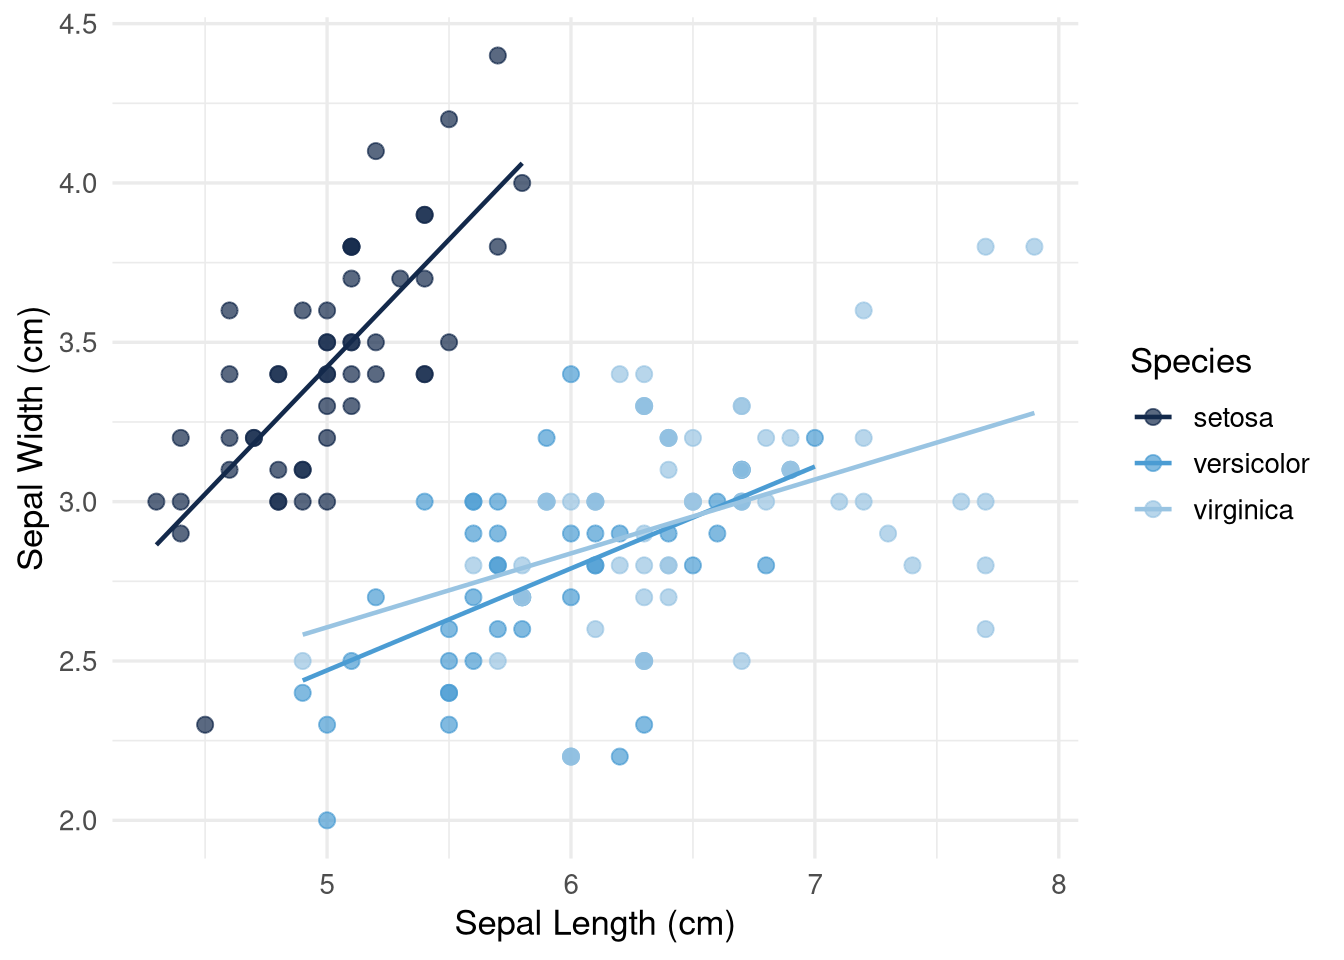
\includegraphics[keepaspectratio]{index_files/figure-latex/notebooks-analysis-fig-iris-sepal-output-2.png}}

}

\caption{\label{fig-iris-sepal}Sepal length vs.~width across three iris
species}

\end{figure}%

\textsubscript{Source:
\href{https://russblessing.github.io/positron-quarto/notebooks/analysis-preview.html\#cell-fig-iris-sepal}{Analysis
Notebook}}

\subsubsection{Petal Length}\label{petal-length}

Species separation is even more pronounced in petal length
(Figure~\ref{fig-iris-petal}), making it a reliable discriminating
variable.

\begin{figure}[H]

\centering{

\pandocbounded{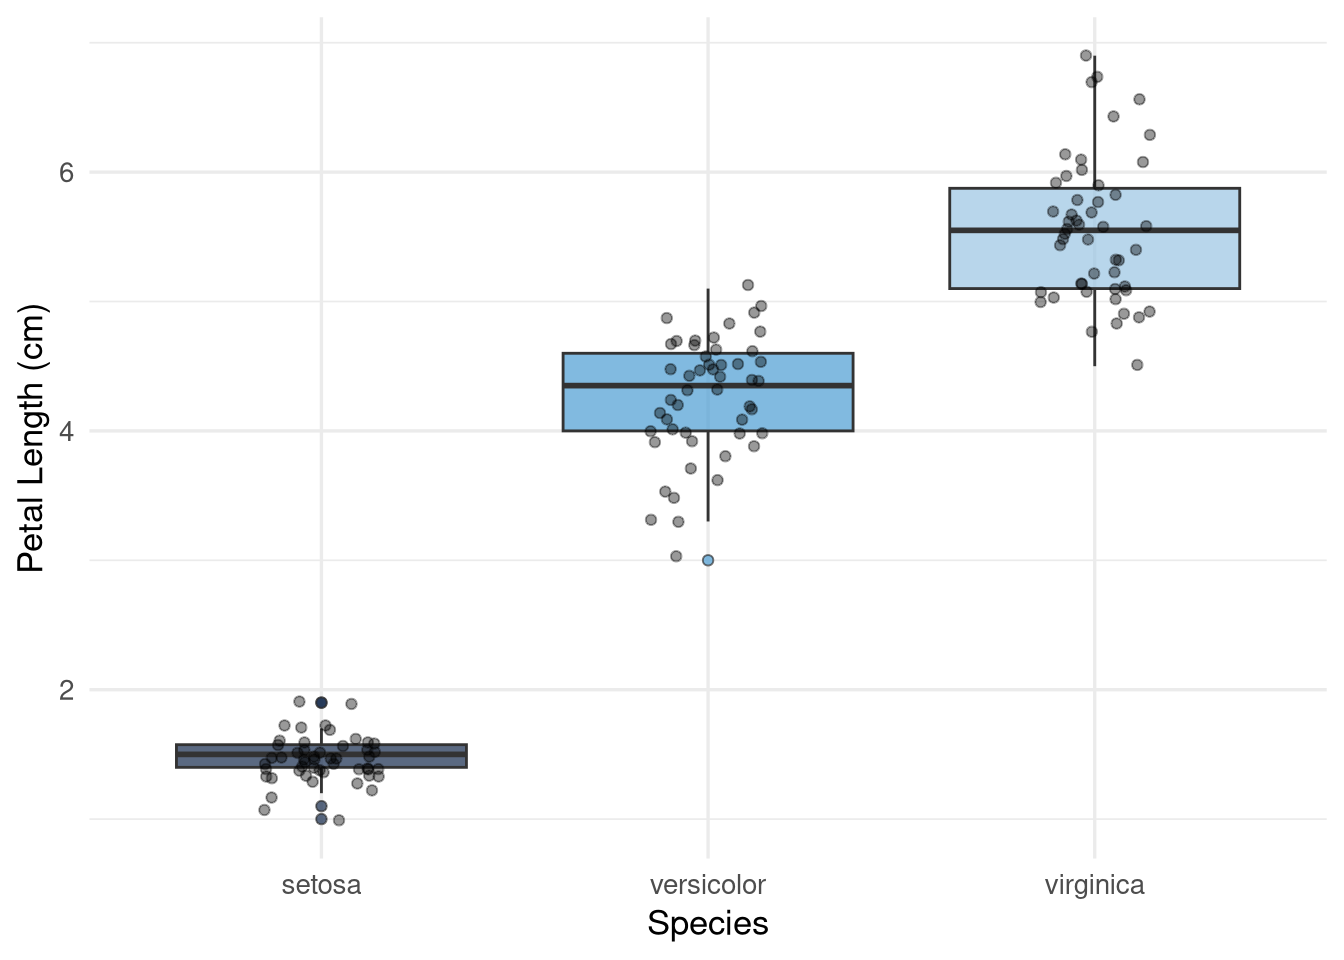
\includegraphics[keepaspectratio]{index_files/figure-latex/notebooks-analysis-fig-iris-petal-output-1.png}}

}

\caption{\label{fig-iris-petal}Distribution of petal length by species}

\end{figure}%

\textsubscript{Source:
\href{https://russblessing.github.io/positron-quarto/notebooks/analysis-preview.html\#cell-fig-iris-petal}{Analysis
Notebook}}

\subsection{Motor Trend Cars}\label{motor-trend-cars}

The \texttt{mtcars} dataset records fuel efficiency and physical
characteristics for 32 automobiles from the 1974 Motor Trend magazine
(Henderson and Velleman 1981). Figure~\ref{fig-mtcars} illustrates the
well-known negative relationship between vehicle weight and fuel
efficiency, stratified by cylinder count.

\begin{figure}[H]

\centering{

\pandocbounded{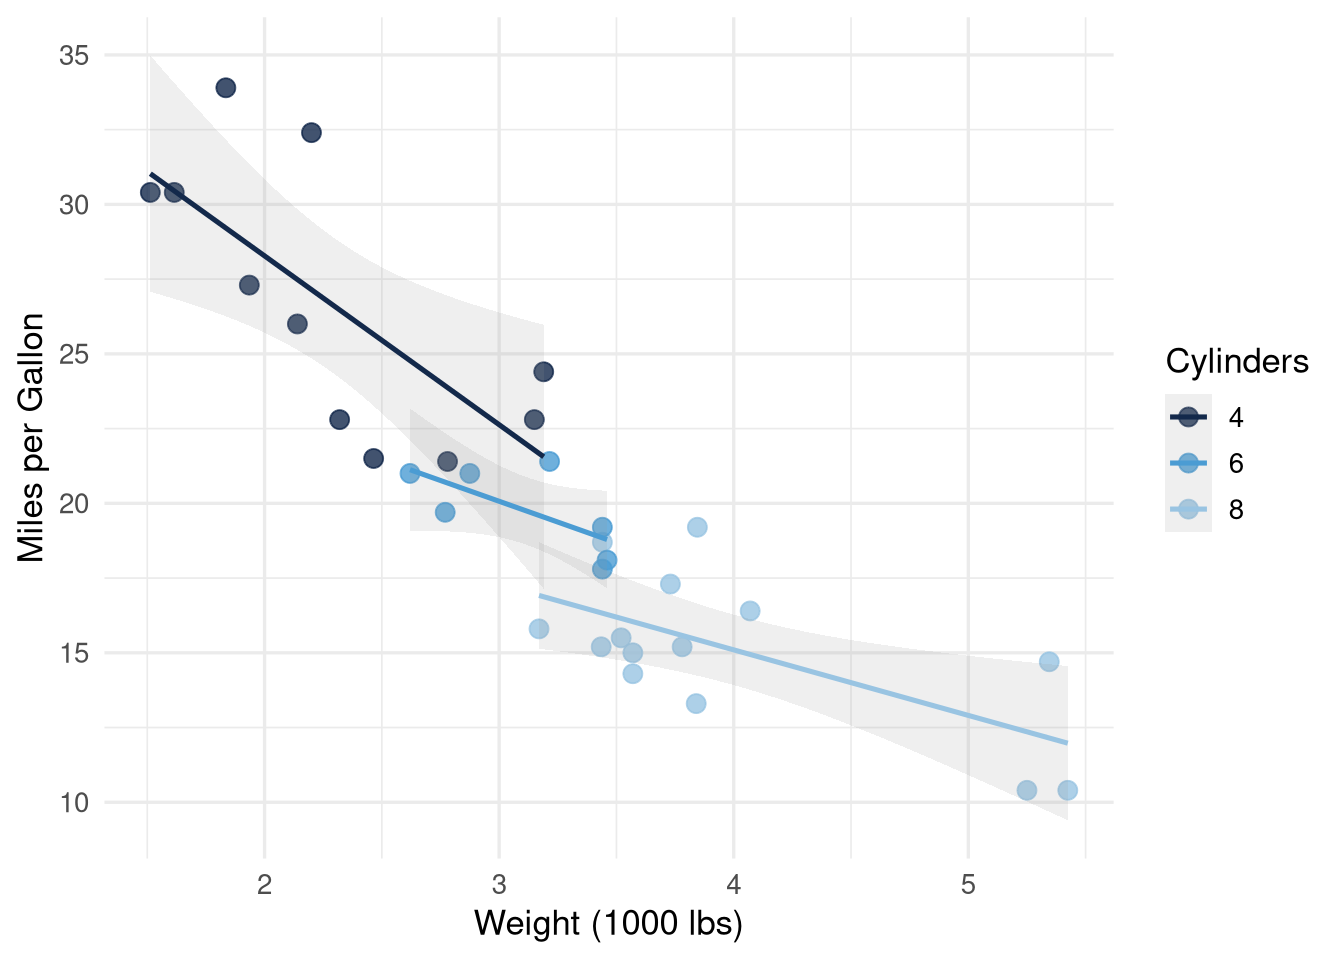
\includegraphics[keepaspectratio]{index_files/figure-latex/notebooks-analysis-fig-mtcars-output-2.png}}

}

\caption{\label{fig-mtcars}Vehicle weight vs.~fuel efficiency, by number
of cylinders}

\end{figure}%

\textsubscript{Source:
\href{https://russblessing.github.io/positron-quarto/notebooks/analysis-preview.html\#cell-fig-mtcars}{Analysis
Notebook}}

\subsection{Conclusion}\label{conclusion}

This document was rendered entirely from plain-text source files. The
figures above were produced in \texttt{notebooks/analysis.qmd} and
embedded without manual copying. Any change to the analysis notebook is
reflected here on the next render.

\subsection*{References}\label{references}
\addcontentsline{toc}{subsection}{References}

\phantomsection\label{refs}
\begin{CSLReferences}{1}{0}
\bibitem[\citeproctext]{ref-anderson1935}
Anderson, Edgar. 1935. {``The Irises of the Gaspe Peninsula.''}
\emph{Bulletin of the American Iris Society} 59: 2--5.

\bibitem[\citeproctext]{ref-henderson1981}
Henderson, Harold V, and Paul F Velleman. 1981. {``Building Multiple
Regression Models Interactively.''} \emph{Biometrics} 37 (2): 391--411.

\end{CSLReferences}




\end{document}
